\chapter{Motivaciones para RG: Relatividad Especial y Gravitaci'on newtoniana}
\section{Distribuci'on de energ'ia y mom'entum de la materia: tensor de energ'ia-mom'entum}

Para un resumen de las definiciones b'asicas, la notaci'on y convenciones usadas en la teor'ia de la mec'anica y electrodin'amica relativista, vea los apuntes de Electrodin\'amica (II) \cite{7}.

En la teor'ia newtoniana de la gravitaci'on la \textit{masa} de los cuerpos es la fuente del campo gravitacional. Desde el punto de vista de una descripci'on de un sistema como un \textit{continuo}, la distribuci'on espacial y el movimiento de su masa es caracterizada por 4 cantidades: la densidad de masa $\rho$ y (las tres componentes de) la densidad de corriente de masa\footnote{Si el sistema est'a constituido de una distribuci'on de densidad $\rho$ que se mueve con velocidad $\vec{v}$, entonces $\vec{J}=\rho\vec{v}$.} $\vec{J}$. En la teor'ia de RE, por otro lado, la masa de los cuerpos no es m'as que una componente de la energ'ia de 'estos: el concepto de masa es reemplazado por el de energ'ia (no existe ley de conservaci'on de la masa de un sistema, sino s'olo de la energ'ia total, etc.). M'as a'un, la energ'ia es ``s'olo'' una componente del 4-mom'entum de un cuerpo. Los valores de las componentes del 4-mom'entum, y por lo tanto de la energ'ia y del mom'entum lineal, se ``mezclan'' al describir un sistema desde distintos SRI's (el 4-mom'entum es un 4-vector bajo TL's). Por todo esto, es natural asumir que en una teor'ia relativista de la gravitaci'on las fuentes del campo gravitacional est'en descritas por la distribuci'on de energ'ia y mom'entum en el espacio(tiempo) y sus flujos\footnote{Es decir, densidad de energ'ia, densidad de flujo de energ'ia, densidad de mom'entum y densidad de flujo de mom'entum.}. Todas estas cantidades quedan condensadas en el \textit{tensor energ'ia-mom'entum de un sistema}.

Las componentes del tensor de energ'ia-mom'entum\footnote{De acuerdo a nuestras convenciones este tensor tiene unidades de \textit{densidad de energ'ia}, es decir, energ'ia por unidad de volumen o, equivalentemente, de \textit{presi'on}.} $T^{\mu\nu}$ est'an relacionadas con las densidades y flujos de energ'ia y mom'entum, de acuerdo a
\begin{equation}
 T^{00}(x)=u(x), \qquad T^{0i}(x)=\frac{1}{c}S^i(x), \qquad T^{i0}(x)=c\,\pi^i(x), \qquad T^{ij}(x)=p^{ij}(x),
\end{equation}
donde $u$ es la \textit{densidad de energ'ia} (energ'ia por unidad de volumen), $S^i$ la \textit{densidad de flujo de energ'ia} (energ'ia por unidad de tiempo y superficie), $\pi^i$ la \textit{densidad de mom'entum} (mom'entum por unidad de volumen) y $p^{ij}$ el \textit{tensor de tensiones} (mom'entum por unidad de tiempo y superficie).

El \textit{4-mom'entum total del sistema}, contenido en un volumen $V$ en un instante dado, es entonces la integral
\begin{equation}
p^\mu=\frac{1}{c}\int_V T^{\mu 0}\,dV \label{pmTmn}
\end{equation}
o, equivalentemente, la energ'ia y el mom'entum adoptan la forma
\begin{equation}
E=\int_V u\,dV, \qquad P^i=\int_V \pi^i\,dV.
\end{equation}
Si el sistema est'a \textit{aislado}, de modo que su energ'ia y mom'entum se conserven, se satisface 
\begin{equation}
 \partial_\nu T^{\mu \nu}=0
\end{equation}
que, en virtud de las identificaciones anteriores, es equivalente a las usuales ``ecuaciones de continuidad'' para la energ'ia y el mom'entum:
\begin{equation}
 \partial_tu+\partial_iS^i=0, \qquad \partial_t \pi^i+\partial_jp^{ij}=0.
\end{equation}


\subsection{Campo electromagn'etico}
El campo electromagn'etico posee y transporta energ'ia y mom'entum. El respectivo tensor de energ'ia-mom'entum del campo electromagn'etico en el vac'io es dado por
\begin{equation}
\boxed{T_\text{em}^{\mu\nu}:=\frac{1}{\mu_0}\left(  F^{\mu\lambda}F_\lambda^{\ \nu}+\frac{1}{4}F_{\rho\sigma}F^{\rho\sigma}\eta^{\mu\nu} \right).}  \label{temsimSI}
\end{equation}
Puede verificarse que las densidades de energ'ia, mom'entum y sus flujos est'an dados por las cantidades apropiadas definidas en electrodin'amica:
\begin{align}
u &:= \frac{1}{2}\left(\varepsilon_0\vec{E}^2+\frac{1}{\mu_0}\vec{B}^2\right),\label{uTheta}\\
S^i &:= \frac{1}{\mu_0}\left(\vec{E}\times\vec{B}\right)^i=c^2\pi^i, \label{STheta}\\
T^{ij} &:= \frac{1}{2}\left(\varepsilon_0\vec{E}^2+\frac{1}{\mu_0}\vec{B}^2\right)\delta_j^i-\varepsilon_0 E^i E^j -\frac{1}{\mu_0}B^i B^j , \label{TTheta}
\end{align}
Para mayores detalles, ver \cite{7}.


\subsection{Fluido perfecto}
Consideramos ahora un fluido con estructura interna descrita por una \textit{presi'on
is'otropa} $p$. 'Esta est'a definida respecto al SRI com'ovil $K'$ con un elemento de fluido dado, ubicado en el evento $x$, de modo que
\begin{eqnarray}
T'^{00}(x)&=&u_0(x) , \label{t00c}\\
T'^{0i}(x) &=&0, \label{t0ic}\\
T'^{i0}(x) &=&0, \label{ti0c}\\
T'^{ij}(x) &=&p(x)\,\delta^{ij} .\label{tijc}
\end{eqnarray}

La componente en (\ref{t00c}) es la \textit{densidad propia de energ'ia} (es decir, $u_0(x)\,dV'$ es la energ'ia del sistema contenida en el elemento de volumen $dV'$, en el SRI instant'aneamente com'ovil con el fluido en el evento $x$), que a menudo se expresa en t'erminos de la \textit{densidad propia de masa} $\rho(x)$, definida por $\rho(x):=u_0(x)/c^2$. Las componentes
mixtas (\ref{t0ic}) y (\ref{ti0c}) son nulas puesto que asumimos que en el sistema com'ovil \textit{la distribuci'on microsc'opica es is'otropa}, por lo que no existe una direcci'on preferente para el flujo de energ'ia ni para la densidad de mom'entum. Finalmente las componentes espaciales
en (\ref{tijc}) son diagonales puesto que \textit{asumimos que en un fluido
perfecto la fuerza sobre cada elemento de superficie es normal a esta
superficie}, de modo que $T^{ij}dS^j=T^{ij}\,\hat{n}^j\,dS=p\,\hat{n}^i dS$ y que $p>0$ corresponde a un fluido que tiende a expandirse.

A partir del tensor de energ'ia-mom'entum para un fluido perfecto en su sistema local com'ovil, encontraremos la expresi'on general respecto a cualquier
otro SRI por medio del boost de Lorentz apropiado. Para esto usaremos los resultados y convenciones contenidos en \cite{7}. Si la TL es denotada como $x'^\mu=\Lambda^\mu_{\ \nu}x^\nu$ y $v^i=c\beta^i$ es la velocidad de $K'$ respecto a $K$ entonces
\begin{equation}
 \Lambda^0_{\ 0}=\gamma, \qquad \Lambda^i_{\ 0}=\Lambda^0_{\ i}=-\gamma\beta^i, \qquad \Lambda^i_{\ j}=\delta^i_j
+\frac{(\gamma-1) }{\beta^2}\beta^i\beta^j .
\end{equation}
Por otro lado el tensor buscado $T^{\mu\nu}$ est'a relacionado con $T'^{\mu\nu}$ por medio de
\begin{eqnarray}
T^{\mu\nu}&=&(\Lambda^{-1})^\mu_{\ \lambda}(\Lambda^{-1})^\nu_{\ \rho}T'^{\lambda\rho}
\\
&=& (\Lambda^{-1})^\mu_{\ 0}\Lambda^\nu_{\ 0}T'^{00}+(\Lambda^{-1})^\mu_{\
i}\Lambda^\nu_{\ j}T'^{ij}\\
&=& (\Lambda^{-1})^\mu_{\ 0}(\Lambda^{-1})^\nu_{\ 0}\rho c^2+p(\Lambda^{-1})^\mu_{\
i}(\Lambda^{-1})^\nu_{\ j}\delta^{ij}.
\end{eqnarray}
Las componentes de la matriz $(\Lambda^{-1})$ est'an dadas por
\begin{equation}
(\Lambda^{-1})^0_{\ 0}=\gamma, \qquad (\Lambda^{-1})^i_{\ 0}=(\Lambda^{-1})^0_{\ i}=+\gamma\beta^i, \qquad (\Lambda^{-1})^i_{\ j}=\delta^i_j
+\frac{(\gamma-1) }{\beta^2}\beta^i\beta^j .
\end{equation}
Por lo tanto, obtenemos que
\begin{eqnarray}
T^{00}&=& (\Lambda^{-1})^0_{\ 0}(\Lambda^{-1})^0_{\ 0}\rho c^2+p(\Lambda^{-1})^0_{\ i}(\Lambda^{-1})^0_{\ j}\delta^{ij} \\
&=& \gamma^2\rho c^2+p\gamma^2\beta^i\beta^j\delta^{ij} \\
&=& \gamma^2\rho c^2+p\gamma^2\beta^2 .
\end{eqnarray}

Vemos que en el contexto de la teor'ia Especial de la Relatividad \textit{la presi'on de un fluido en movimiento aporta a su densidad de energ'ia}\footnote{En su generalizaci'on a la teor'ia General de la Relatividad, este hecho tiene importantes consecuencias, por ejemplo, para el an'alisis de estabilidad (y colapso) estelar.}. Adem'as,
\begin{eqnarray}
T^{0i}&=& (\Lambda^{-1})^0_{\ 0}(\Lambda^{-1})^i_{\ 0}\rho c^2+p\,(\Lambda^{-1})^0_{\ j}(\Lambda^{-1})^i_{\ k} \delta^{jk} \\
&=& \gamma^2\beta^i\rho c^2 +p\gamma\beta^j\left(\delta^i_k
+\frac{1}{\beta^2}\beta^i\beta^k(\gamma-1) \right) \delta^{jk} \\
&=& \gamma^2\beta^i\rho c^2 +p\gamma\left(\beta^i +\beta^i(\gamma-1) \right)
\\
&=& \gamma^2\beta^i\rho c^2 +p\gamma^2\beta^i,
\end{eqnarray}
y $T^{i0}=T^{0i}$. Note adem'as que $T^{0i}\neq T^{00}\beta^i$ cuando $p\neq 0$. Finalmente,
\begin{eqnarray}
T^{ij}&=& (\Lambda^{-1})^i_{\ 0}(\Lambda^{-1})^j_{\ 0}\rho c^2+p\,(\Lambda^{-1})^i_{\ k}(\Lambda^{-1})^j_{\ l}\delta^{kl} \\
&=&\gamma^2\beta^i\beta^j\rho c^2+ p\left(\delta^i_k+
\frac{1}{\beta^2}\beta^i\beta^k(\gamma-1) \right)\left(\delta^j_l
+\frac{1}{\beta^2}\beta^j\beta^l(\gamma-1) \right)\delta^{kl} \\
&=&\gamma^2\beta^i\beta^j\rho c^2+p\left(\delta^{ij}
+\frac2{\beta^2}\beta^i\beta^j(\gamma-1)
+\frac{1}{\beta^2}\beta^i\beta^j(\gamma-1)^2\right) \\
&=&\gamma^2\beta^i\beta^j\rho c^2+p\left(\delta^{ij}
+\frac{1}{\beta^2}\beta^i\beta^j(\gamma^2-1)\right) \\
&=&\gamma^2\beta^i\beta^j\rho c^2+p\left(\delta^{ij}
+\gamma^2\beta^i\beta^j\right).
\end{eqnarray}
Puede verificarse f'acilmente que 'estas son precisamente las componentes de
\begin{equation}\label{temfp}
\boxed{T_{\rm fp}^{\mu\nu}=\left( \rho +\frac{p}{c^2}\right) u^\mu
u^\nu-p\,\eta^{\mu\nu}.}\marginnote{energ'ia-mom'entum fluido perfecto}
\end{equation}

La expresi'on (\ref{temfp}) constituye por tanto la expresi'on covariante del tensor de energ'ia-mom'entum de un fluido perfecto, caracterizado por su densidad propia de masa $\rho$, y su presi'on is'otropa $p$, movi'endose con 4-velocidad $u^\mu$. Estas tres cantidades son, en general, dependientes de la posici'on y del tiempo. En t'erminos de la densidad propia de energ'ia, $u_0$, tenemos:
\begin{equation}\label{temfpu}
\boxed{T_{\rm fp}^{\mu\nu}=\left(u_0 +p\right)\frac{u^\mu}{c}
\frac{u^\nu}{c}-p\,\eta^{\mu\nu}.}\marginnote{energ'ia-mom'entum fluido perfecto}
\end{equation}
\subsection{Fluido simple (polvo)}

El caso particular de un fluido simple, es decir, sin presi'on, describe la situaci'on en que el sistema est'a constituido por  un conjunto de part'iculas \textit{no interactuantes movi'endose todas con la misma velocidad} en un elemento de volumen dado (``polvo''). El tensor energ'ia-mom'entum se reduce entonces a:
\begin{equation}
\boxed{T_{\rm polvo}^{\mu\nu}(x)=\rho\, u^\mu u^\nu.}
\end{equation}

Las respectivas densidades de energ'ia, de flujo de energ'ia, de mom'entum y el
tensor de tensiones est'an dadas en este caso por:
\begin{eqnarray}
u&=&\rho \gamma^2 c^2, \\ 
S^i&=&\rho \gamma^2c^2v^i=u\,v^i, \\ 
{\pi}^i&=&\rho \gamma^2v^i =\frac{u}{c^2}v^i, \\ 
p^{ij} &=&\rho \gamma^2 v^i v^j=\pi^iv^j.
\end{eqnarray}
Note que para este tipo de sistema se verifica que los respectivos flujos $S^i$ y $p^{ij}$ tienen la forma esperada de producto de la respectiva densidad (``transportada'') y la velocidad de cada elemento de fluido (``a la que es transportada''), tal como ocurre por ejemplo para una distrubuci'on de carga de densidad $\rho_{\rm c}$ movi'endose con velocidad $\vec{v}_{\rm c}$, para la cual la densidad de corriente es dada por $\vec{J}_{\rm c}=\rho_{\rm c}\vec{v}_{\rm c}$.

\section{Ley de Gravitaci'on universal}
En la teor'ia newtoniana la fuerza gravitacional de una masa muy peque\~na (``puntual'') $m_1$ sobre otra masa (tambi'en muy peque\~na) $m_2$
est'a dada por la ley de gravitaci'on de Newton ($1687$),
\begin{equation}
\vec{F}_{1\rightarrow 2}=-G\frac{m_1m_2}{|\vec{r}|^2}\frac{\vec{r}}{|\vec{r}|},
\end{equation}
donde $G$ es la constante de gravitaci'on (de Cavendish, medida por primera vez en 1897). Su valor, de acuerdo a las mediciones actuales, es\footnote{Ver por ejemplo, \url{http://www.codata.org}.}
\begin{equation}
G\stackrel{\rm SI}{=}(6,674 28\pm 0.000 67)\times 10^{-11}\, m^3kg^{-1}s^{-2}.
\end{equation}
El vector $\vec{r}:=\vec{x}_2-\vec{x}_1$ apunta desde $m_1$ hasta $m_2$, ver figura \ref{lguN}. De acuerdo al principio de acci'on y reacci'on (tercera ley de Newton),
tenemos que $\vec{F}_{1\rightarrow 2}=-\vec{F}_{2\rightarrow 1}$.
\begin{center}
\begin{figure}[H]
\centerline{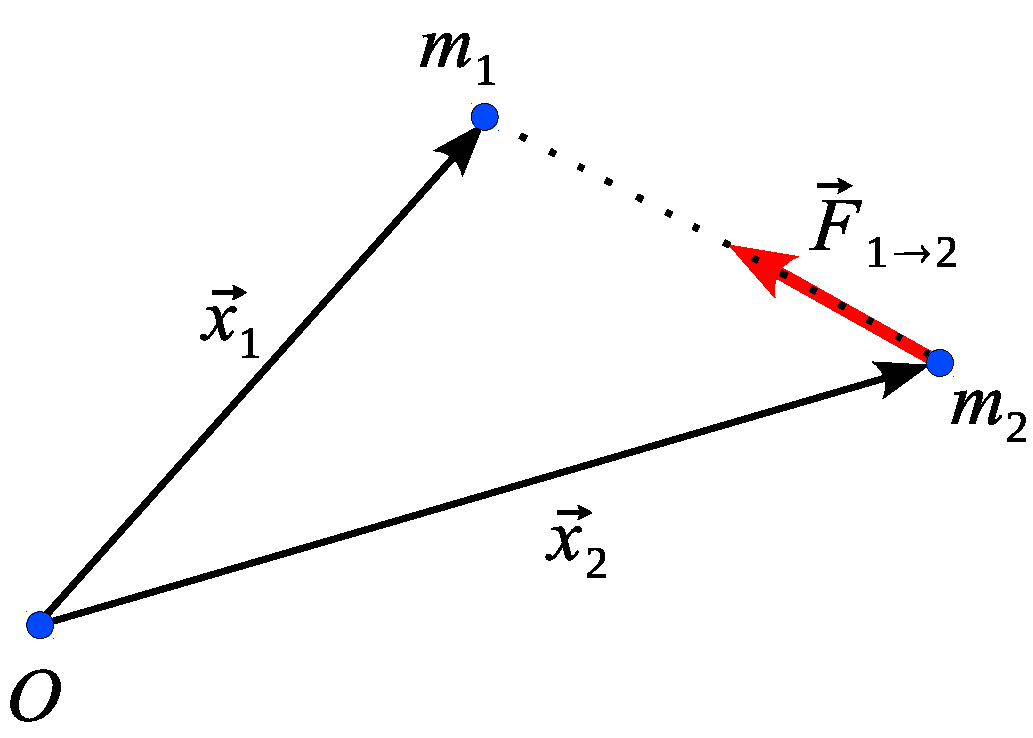
\psfig{file=fig/fig-ley-gravitacion-Newton.pdf,height=4cm,angle=0}}
\caption{Ley de gravitaci'on universal de Newton.}
\label{lguN}
\end{figure}
\end{center}
El \textit{campo gravitacional} $\vec{g}$ es definido como la fuerza por unidad de masa
que experimenta una masa de prueba. Por tanto, el campo gravitacional en la posici'on $\vec{x}_2$ generado por una masa (muy peque\~na) $m_1$ es
\begin{equation}
\vec{g}_1(x_2):=\frac{\vec{F}_{1\to 2}}{m_2}=-G\frac{m_1}{|\vec{r}|^2}\frac{\vec{r}}{|\vec{r}|}.
\end{equation}
En el caso anterior, es posible distinguir entre la masa $m_1$ que
\textit{genera} el campo gravitacional, que llamamos \textit{masa gravitacional
activa}, y la masa $m_2$ de la part'icula que sobre la cual act'ua la fuerza, que
llamaremos \textit{masa gravitacional pasiva}.

Por el \textit{principio} de superposici'on, el campo gravitacional generado por una distribuci'on continua de masa, caracterizada por su densidad de masa $\rho(\vec{x})$ ser'a de la forma
\begin{equation}
\vec{g}(\vec{x})=-G\int_V\frac{\rho(\vec{x}')(\vec{x}-\vec{x}')}{|\vec{x}-\vec{x}'|^3}dV'.
\end{equation}
Como consecuencia, el campo gravitacional es siempre irrotacional,
\begin{equation}
\vec{\nabla}\times\vec{g}=\vec{0},
\end{equation}
y puede derivarse a partir de un \textit{potencial gravitacional} $\phi$, de modo
que
\begin{equation}
\boxed{\vec{g}(x)=-\vec{\nabla}\phi(x),}
\end{equation}
donde
\begin{equation}
\phi(\vec{x}):=-G\int_V\frac{\rho(\vec{x}')}{|\vec{x}-\vec{x}'|}dV'+\text{cte}.
\end{equation}
Este potencial satisface la \textit{ecuaci'on de Poisson},
\begin{equation}\marginnote{Ecuaci'on de Poisson}
\boxed{\nabla^2\phi=4\pi G \rho,} \label{Poisson}
\end{equation}
o equivalentemente, el campo gravitacional satisface la ecuaci'on (``de Gauss")
\begin{equation}
\vec\nabla\cdot\vec{g}=-4\pi G \rho, \label{gaussg}
\end{equation}
que relaciona los \textit{gradientes} del campo gravitacional con la distribuci'on de masa, descrita por la densidad $\rho(\vec{r})$, que lo genera.

Si bien la ecuaci'on (\ref{Poisson}) es una ecuaci'on para el campo $\phi$, en el
contexto newtoniano el campo gravitacional no es un genuino \textit{campo
din'amico}, es decir, no contiene grados de libertad independientes, ya que
'este queda determinado (para condiciones de borde dadas) 'unicamente por la
densidad de masa $\rho$. En otras palabras, la teor'ia newtoniana de la
gravitaci'on es una teor'ia de \textit{acci'on a distancia}. De acuerdo a este modelo, si se removiese la fuente del campo ($\rho\rightarrow 0$) entonces el campo gravitacional desaparecer'ia \textit{instant'aneamente} en todo punto. El mismo Newton estaba bastante preocupado por este hecho. Claramente, esta propiedad es \textit{incompatible} con los postulados b'asicos de la teor'ia de Relatividad Especial.

\section{Masa inercial y masa gravitacional}
Una caracter'istica especial de la interacci'on gravitacional es que la
aceleraci'on de un cuerpo que cae libremente en un campo gravitacional dado \textit{no depende de su masa sino s'olo de su posici'on} en el campo gravitacional. En el contexto newtoniano esto puede describirse a trav'es de la igualdad entre la \textit{masa inercial} y la \textit{masa gravitacional} de \textit{todo cuerpo}.

En este contexto, la \textit{masa inercial} de un cuerpo, $\stackrel{\rm iner}{m}$, es definida como aquella cantidad que mide la resistencia de 'este a cambiar su estado de movimiento, de acuerdo a la segunda ley de Newton:
\begin{equation}\label{2ln}
\vec{F}=\stackrel{\rm iner}{m}\frac{d^2\vec{x}}{dt^2}.
\end{equation}
Esta masa puede ser determinada por medio de experimentos ``no-gravitacionales'', es decir, que no involucran la interacci'on gravitacional. Por ejemplo, puede determinarse la masa inercial de un cuerpo comparando su frecuencia de oscilaci'on $\omega$ con la frecuencia de oscilaci'on de un cuerpo de referencia $\omega_{\rm ref}$) cuando ambos son unidos alternativamente a un mismo resorte, de modo que se produzca una oscilaci'on horizontal. En este caso (asumiendo la ley de Hooke) se cumple que $\stackrel{\rm iner}{m}/\stackrel{\rm iner}{m}_{\rm ref}=\omega_{\rm ref}^2/\omega^2$.

Por otro lado, se define la \textit{masa gravitacional}, $\stackrel{\rm grav}{m}$, de un cuerpo como la cantidad que mide la magnitud de la fuerza que este cuerpo experimenta al estar en una regi'on del espacio con campo gravitacional $\vec{g}$:
\begin{equation}\label{fg}
\vec{F}_{\rm grav}=\stackrel{\rm grav}{m}\vec{g}=-\stackrel{\rm grav}{m}\vec\nabla\phi.
\end{equation}
A partir de (\ref{2ln}) y (\ref{fg}) obtenemos que la aceleraci'on de un cuerpo debido a un campo gravitacional $\vec{g}$ es dado por
\begin{equation}\label{amimg}
\frac{d^2\vec{x}}{dt^2}=\left(\frac{\stackrel{\rm grav}{m}}{\stackrel{\rm iner}{m}}\right)\vec{g}.
\end{equation}
Esta expresi'on es an'aloga a la que determina la aceleraci'on de un cuerpo cargado en presencia de un campo el'ectrico externo:
\begin{equation}\label{aqE}
\frac{d^2\vec{x}}{dt^2}=\left(\frac{q}{\stackrel{\rm iner}{m}}\right)\vec{E}.
\end{equation}
En este sentido, la masa gravitacional es el an'alogo gravitacional a la carga el'ectrica (es decir, es la ``carga gravitacional'').


\subsection{Universalidad de la interacci'on gravitacional, Principio de Equivalencia D'ebil}

La experiencia muestra que la interacci'on electrost'atica causa, incluso en presencia de un mismo campo el'ectrico, que cuerpos diferentes aceleren en forma diferente. Esto se describe, de acuerdo a (\ref{aqE}), diciendo que distintos cuerpos poseen distintos valores de la relaci'on carga-masa (inercial) $q/m$. Existen cuerpos donde esta relaci'on es positiva, negativa, o cero. En contraste, la interacci'on gravitacional \textit{parece} (de acuerdo a todas observaciones realizadas hasta hoy) tener la propiedad 'unica que \textit{todos} los cuerpos aceleran en la \textit{misma} direcci'on y con la \textit{misma} magnitud en un campo gravitacional dado. De acuerdo a (\ref{amimg}), esto requiere que el cuociente entre la masa inercial y gravitacional de todo cuerpo sea una constante universal (es decir, que tenga siempre el mismo valor). Por simplicidad, usualmente se eligen las unidades de $\stackrel{\rm grav}{m}$ (o, equivalentemente, de la constante gravitacional $G$) tal que esta \textit{universalidad de la interacci'on gravitacional} implique que
\begin{equation}
\boxed{\stackrel{\rm iner}{m}=\stackrel{\rm grav}{m}.}
\end{equation}
En este caso, (\ref{amimg}) se reduce a
\begin{equation}\label{ag}
\frac{d^2\vec{x}}{dt^2}=\vec{g}
\end{equation}
\textit{para todo cuerpo}.

Si el \textit{postulado} de universalidad de la interacci'on gravitacional o, en otras palabras, de la igualdad de masa inercial y gravitacional, es \textit{siempre} v'alido entonces la trayectoria de los cuerpos sometidos (s'olo) a la acci'on de la gravedad es independiente del cuerpo (de su carga, composici'on, temperatura, color, etc.) y s'olo depende del campo gravitacional en el que se encuentra (determinado por los otros cuerpos en el sistema) y de la posici'on y velocidad inicial de 'este. La suposici'on que las trayectorias de los cuerpos sometidos a la acci'on de la gravedad son realmente id'enticas (dadas las mismas condiciones iniciales) es usualmente llamado \textbf{Principio de Equivalencia D'ebil} (PED). Lo importante es que la validez del PED o, equivalentemente, de la universalidad de la aceleraci'on debido a la gravedad, o de la igualdad de las masas inerciales y gravitacionales, son caracter'isticas distintivas de la interacci'on gravitacional que se han obtenido a partir de la generalizaci'on de \textit{observaciones}, y que pueden (y deben!) ser testeadas experimentalmente. Hasta ahora, toda la evidencia observacional respalda al PED. Estas observaciones abarcan desde los experimentos originales de Galileo usando p'endulos, planos inclinados, etc. hasta los m'as modernos y precisos experimentos con sat'elites e incluso neutrones \cite{Koester76} y electrones. A la fecha, el PED ha sido verificado con precisiones que restringen las posibles \textbf{desviaciones relativas de la aceleraci'on}, y por lo tanto la diferencia relativa del cuociente $\stackrel{\rm iner}{m}/\stackrel{\rm grav}{m}$ entre dos cuerpos (``1'' y ``2'')
\begin{equation}
\frac{\Delta a}{a}=\frac{\left(\stackrel{\rm iner}{m}/\stackrel{\rm grav}{m}\right)_2-\left(\stackrel{\rm iner}{m}/\stackrel{\rm grav}{m}\right)_1}{\left(\stackrel{\rm iner}{m}/\stackrel{\rm grav}{m}\right)_1},
\end{equation}
a ser menores que una parte en $10^{13}$. Para m'as detalles, ver \cite{Will06}-\cite{STEP}. Como veremos m'as adelante, la teor'ia general de la relatividad de Einstein \textit{asume} como ingrediente crucial para su construcci'on el PED\footnote{de hecho se asume una versi'on generalizada y a'un m'as demandante, el as'i llamado ``principio de equivalencia fuerte'' (PEF).}. Por esta raz'on existe continuo interer'es en poner a prueba este principio, y mejorar cada vez m'as la precisi'on con la que se ha verificado su validez.

El siguiente gr'afico resume los resultados de m'ultiples experimentos modernos que determinan cotas m'aximas para las aceleraciones relativas de distintos cuerpos sometidos a la acci'on de la gravedad, junto con el a\~no en que fueron realizados los experimentos.
\begin{center}
\begin{figure}[H]
\centerline{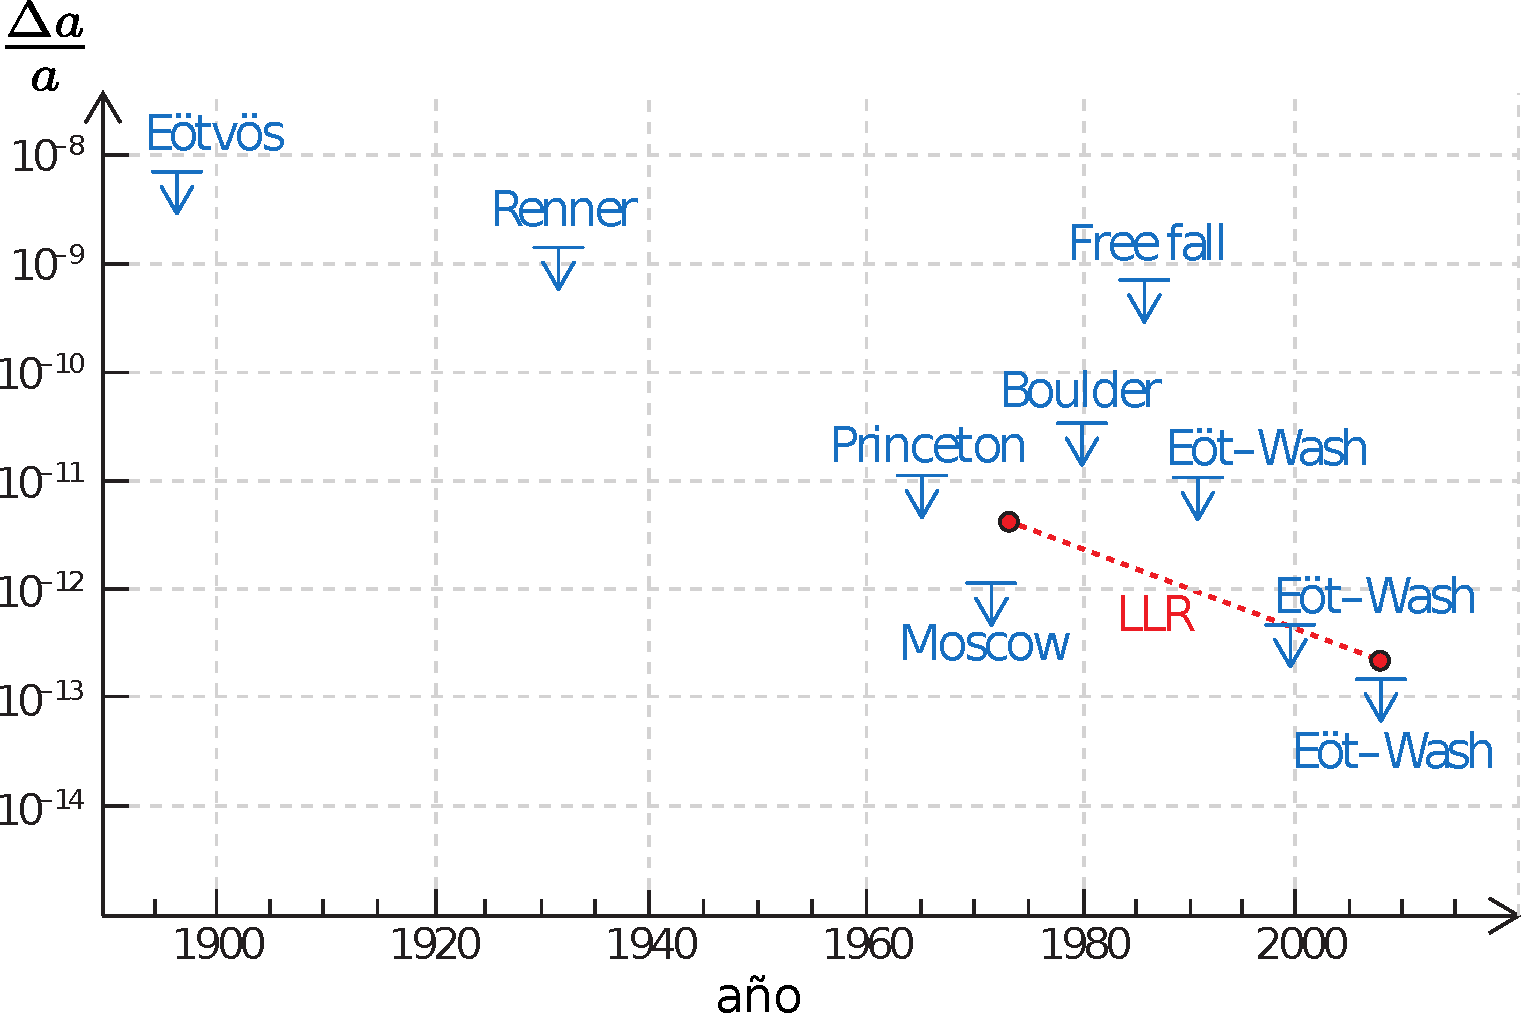
\psfig{file=fig/fig-tests-PED.pdf,height=5cm,angle=0}}
\caption{L'imites a posibles violaciones del PED. Figura adaptada a partir de la original en \cite{Turyshev08}.}
\label{fig:equiv1}
\end{figure}
\end{center}

\section{Fuerzas de marea}
%Tal como hemos visto, un indicador de la presencia de campo gravitacional no nulo es la \textit{aceleraci'on relativa} entre distintos SRLI's. 
En el contexto newtoniano, se usa el t'ermino \textit{fuerzas de marea} para describir el efecto de la \textit{inhomogeneidad} de un campo gravitacional, que genera diferencias en la aceleraci'on de la materia en distintas partes de un sistema. Considere el caso de un campo gravitacional generado por una distribuci'on compacta de masa (ver, por ejemplo, la figura \ref{fig:SRLI}). Debido a las inhomogeneidades del campo gravitacional, dos peque\~nas masas de prueba inicialmente en reposo caer'an hacia el centro de fuerzas, acerc'andose entre ellas. Similarmente, una gota de agua inicialmente esf'erica tender'a a deformarse a una forma elipsoidal debido a que la fuerza gravitacional en su parte inferior (m'as cerca del centro de fuerzas) es mayor que en la parte superior, que est'a a una distancia mayor de la fuente.

Si la distancia entre las dos masas de prueba es \emph{suficientemente peque\~na}, podemos encontrar una expresi'on expl'icita simple para su aceleraci'on relativa. Considere que las posiciones de estas masas son $\vec{x}$ y $\vec{x}+\delta\vec{x}$.
Podemos entonces, a primer orden en $\delta\vec{x}$, escribir:
\begin{equation}
a_i(\vec{x}+\delta\vec{x})=a_i(\vec{x})+\delta x^j\partial_j a_i(\vec{x}).
\end{equation}
Esta aproximaci'on es buena si $|\delta\vec{x}|\ll |a_i|/|\partial_j
a_i|$. Definimos el \textit{tensor de mareas} $K_{ij}$ por
\begin{equation}\marginnote{Tensor de Mareas}
K_{ij}(\vec{x}):=-\partial_j a_i(\vec{x}),
\end{equation}
(el signo negativo es convencional) de modo que
\begin{equation}
\delta a_i:=a_i(\vec{x}+\delta\vec{x})-a_i(\vec{x})=- K_{ij}\delta x^j.
\end{equation}
Si ahora expresamos la aceleraci'on relativa en t'erminos de la variaci'on de la posici'on relativa, es decir, $\delta a_i=d^2(\delta x^i)/dt^2$, encontramos 
\begin{equation}\label{desvrel}
\frac{d^2(\delta x^i)}{dt^2}+K_{ij}\delta x^j=0.
\end{equation}
Adem'as, el car'acter irrotacional del campo gravitacional es equivalente a la simetr'ia
del tensor de mareas, $K_{ij}=K_{ji}$. Adem'as,
\begin{equation}
K_{ij}=\partial_i\partial_j\phi.
\end{equation}
En t'erminos de $K$, la ecuaci'on de Poisson (\ref{Poisson}) puede escribirse como
\begin{equation}\label{Kiirho}
%\sum_{i=1}^3
K_{ii}=4\pi G\rho.
\end{equation}
Como veremos posteriormente, el tensor de mareas es el an'alogo newtoniano del \textit{tensor de curvatura de Riemann}, y las relaciones \eqref{desvrel} y \eqref{Kiirho} corresponden al l'imite no-relativista de la \textit{ecuaci'on de desv'io geod'esico} y de las \textit{ecuaciones de Einstein}, respectivamente.



\section{Observadores acelerados y gravedad: Versi'on no-rela\-ti\-vis\-ta}
Considere, a'un en el contexto de la mec'anica de Newton, una part'icula movi'endose s'olo bajo la acci'on de un campo gravitacional $\vec{g}$. Siempre es posible considerar una regi'on suficientemente peque\~na del espacio y un intervalo de tiempo suficientemente corto que permitan aproximar a $\vec{g}$ como \textit{homog'eneo e independiente del tiempo} en aquella regi'on. Como vimos anteriormente, asumiendo la validez del PED, la ecuaci'on de movimiento de toda part'icula respecto de un SRI $K$ ser'a
\begin{equation}\label{enmp}
\frac{d^2\vec{x}}{dt^2}=\vec{g},
\end{equation}
cuya soluci'on es una trayectoria parab'olica:
\begin{equation}\label{tr1}
\vec{x}(t)=\vec{x}_0+\vec{v}_0t+\frac{1}2\vec{g}t^2.
\end{equation}

Considere ahora un SR $K'$ que \textit{acelera respecto a} $K$, con aceleraci'on constante $\vec{a}$. Consideraremos que la transformaci'on entre las coordenadas asociadas a ambos SR's es 
\begin{equation}\label{tgan}
t'=t, \qquad \vec{x}'=\vec{x}-\frac{1}2\vec{a}t^2.
\end{equation}
Verificamos que nuestra interpretaci'on es consistente ya que los eventos sobre trayectorias en reposo respecto a $K'$, es decir, con $\vec{x}'=\vec{x}'_0$, describen un movimiento uniformemente acelerado respecto al SRI $K$: $(ct,\vec{x})=(ct,\vec{x}'_0+\vec{a}t^2/2)$.

Usando la transformaci'on \eqref{tgan} y la aceleraci'on \eqref{enmp} podemos calcular la aceleraci'on de la part'icula respecto a $K'$, obteniendo
\begin{equation}\label{acelprima}
\frac{d^2\vec{x}'}{dt'^2}=\vec{g}-\vec{a}.
\end{equation}
Equivalentemente, la trayectoria respecto a $K'$ es determinada transformando  \eqref{tr1}:
\begin{equation}
\vec{x}'(t)=\vec{x}_0+\vec{v}_0t+\frac{1}2(\vec{g}-\vec{a})t^2.
\end{equation}
\begin{center}
\begin{figure}[H]
\centerline{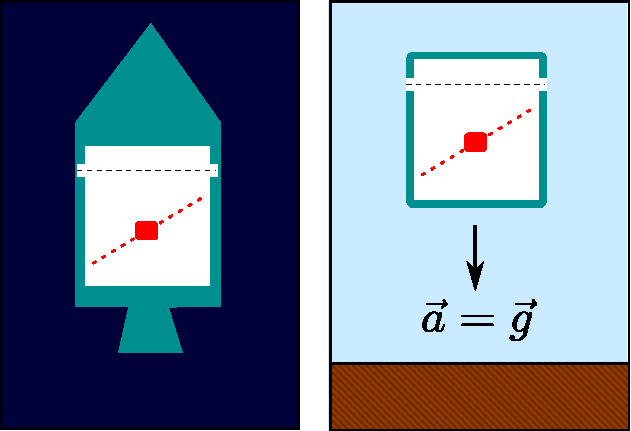
\psfig{file=fig/fig-equivalencia.pdf,height=4cm,angle=0}}
\caption{Equivalencia entre un SRI en ausencia de gravedad y un SR en caida libre.}
\label{fig:equiv2}
\end{figure}
\end{center}

Este resultado establece cierta relaci'on de \textit{equivalencia} en lo que respecta a la mec'anica (es decir, al movimiento de cuerpos) en campos gravitacionales \textit{estacionarios y homog'eneos} y en \textit{SR's acelerados}. Por ejemplo, en un sistema de referencia \textit{en ca'ida libre}, es decir, con $\vec{a}=\vec{g}$, tendremos que cada part'icula describir'a una trayectoria rectil'inea con velocidad constante respecto a $K'$, \textit{tal como lo har'ia en un SRI en el que no existiese campo gravitacional}. Ver figura \ref{fig:equiv1}.
En otras palabras, parece posible ``eliminar'' los efectos de un campo gravitacional (estacionario y homog'eneo) sobre el movimiento de cuerpos, refiriendo estos movimientos a un SR en ca'ida libre\footnote{Ver, por ejemplo, el siguiente \href{http://youtu.be/1ieR8hIXUIg}{video} y tambi'en \href{http://youtu.be/xsNFqMtNZvI}{\'este}.}.
An'alogamente, si consideramos una regi'on muy lejos de todo cuerpo masivo que genere un campo gravitacional ($\vec{g}=\vec{0}$), entonces es posible ``simular'' (los efectos mec'anicos de) un campo gravitacional (estacionario y homog'eneo) describiendo los movimientos desde un SR acelerado (por ejemplo, con aceleraci'on $\vec{a}=-\vec{g}$). Ver figura\footnote{Adaptada a partir de  \href{http://commons.wikimedia.org/wiki/File:Elevator_gravity.svg}{esta} figura original.} \ref{fig:gya}.
\begin{figure}[H]
 \begin{center}
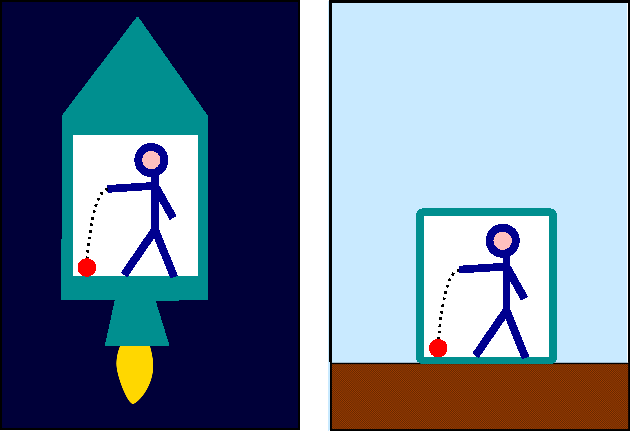
\includegraphics[height=4cm]{fig/fig-gravedad-y-aceleracion.pdf}
\caption{Equivalencia entre campo gravitacional y aceleraci'on.}
\label{fig:gya}
\end{center}
\end{figure}
Note que la existencia de esta equivalencia entre efectos gravitacionales y efectos inerciales depende crucialmente del car'acter universal de la interacci'on gravitacional (en otras palabras, de la validez del PED).

\section{Principio de Equivalencia de Einstein y Sistemas de Referencia Localmente inerciales}
Tal como hemos discutido, la experiencia suministra evidencia a favor de que la interacci'on gravitacional posee las siguientes caracter'isticas:
\begin{quotation}
En una regi'on (espacio-temporal) suficientemente peque\~na (donde las inhomogeneidades del campo puedan ser despreciadas), y respecto a un SR \textit{en ca'ida libre}, las trayectorias de \textit{todo} (peque\~no) cuerpo, libre de fuerzas no-gravitacionales, \textit{son l'ineas rectas con velocidad constante}.
\end{quotation}

Note adem'as que suficientemente lejos de otras distribuciones de masa, donde el campo gravitacional pueda considerarse como nulo, los SR's en ca'ida libre son los usuales SRI's. En este sentido, al menos en lo que respecta a la trayectoria de cuerpos no sometidos a fuerzas no-gravitacionales, los SR's en ca'ida libre juegan el mismo rol f'isico que los SRI's en ausencia de gravedad. Einstein asumi'o que estos SR's en ca'ida libre son \textit{en toda situaci'on}, es decir\marginnote{Principio de Equivalencia de Einstein}, \textit{para todo tipo de fen'omeno f'isico} (no s'olo mec'anico, tambi'en por ejemplo, electromagn'etico), equivalentes a los SRI's en ausencia de gravitaci'on. Por esta raz'on, y dada la extensi'on finita de estos SR's en ca'ida libre, 'estos son tambi'en llamados \textbf{Sistemas de Referencia Localmente Inerciales} (SRLI's). Este supuesto es tambi'en llamado \textbf{Principio de Equivalencia Fuerte} (PEF), en contraste al PED, que se refiere s'olo a la \emph{mec'anica} de los cuerpos (macrosc'opicos).

La primera referencia conocida al PEF se encuentra en el art'iculo de 1907 de Einstein \cite{Einstein07}, cuyo t'itulo podr'ia traducirse ``Sobre el Principio de Relatividad y las consecuencias que de 'el se desprenden".
 Casi al final de este trabajo (p'agina 454) Einstein escribe 
\begin{quotation}
``Wir... wollen ... in folgenden die v\"ollige physikalische Gleichwertigkeit von Gravitationsfeld und entsprechender Beschleunigung des Bezugssystems annehmen",
\end{quotation}
que se traducir'ia como ``queremos asumir la completa equivalencia f'isica de un campo gravitacional y la correspondiente aceleraci'on del sistema de referencia". Acto seguido (en el resto del paper) Einstein estudia las primeras consecuencias de esta suposici'on.
 
El PEF obliga a repensar la existencia y el rol de los Sistemas de Referencia Inerciales. En la mec'anica de Newton y en RE los SRI's juegan un papel fundamental. Un SRI es entendido como un sistema de ejes rectos ortogonales respecto a los cuales un cuerpo libre de fuerzas externas se mueve en l'inea recta con velocidad constante. Esta abstracci'on resulta entonces ser consistente y 'util s'olo en ausencia de interacci'on gravitacional. En presencia de gravitaci'on, por otro lado, \textit{no existen SRI's con extensi'on infinita}. Esto es debido a que, por un lado, de acuerdo al PED, \textit{todas} las trayectorias de cuerpos son afectadas por la gravedad, es decir, no existen cuerpos libres de esta interacci'on. Adem'as, en presencia de campos gravitacionales (no homog'eneos) no existe ning'un SR (``r'igido'' y de extensi'on infinita) respecto al cual los cuerpos se muevan en forma rectil'inea y uniforme.
Sin embargo, en presencia de gravitaci'on los SRLI's s'i tienen realidad f'isica, pero necesariamente tienen una extensi'on finita en el espaciotiempo.
Como los fen'omenos f'isicos no-gravitacionales conocidos son descritos exitosamente en el marco de la Teor'ia Especial de la Relatividad, Einstein asumi'o en su teor'ia de Relatividad General, que incorpora la gravitaci'on, que \textit{es en los SRLI's en ca'ida libre donde son v'alidas las leyes conocidas en la teor'ia de RE}.

En resumen, en presencia de un campo gravitacional general no existen SRI's \emph{globales} (de extensi'on infinita). No obstante, de acuerdo al PEF s'i es posible encontrar SR's en regiones peque\~nas (los SRLI's, es decir, SR's en ``caida libre'') donde las leyes de RE son v'alidas. Un campo gravitacional no nulo est'a entonces caracterizado por el hecho que los SRLI's no pueden ``unirse'' para formar un SRI global. Adem'as, si bien en un SRLI no es posible detectar efectos de la gravedad, s'i es posible hacerlo comparando cantidades f'isicas en \textit{distintos} SRLI's. Por ejemplo, en presencia de campo gravitacional no nulo los SRLI's \textit{aceleran entre s'i}, ver figura \ref{fig:SRLI}.
\begin{figure}[H]
\centering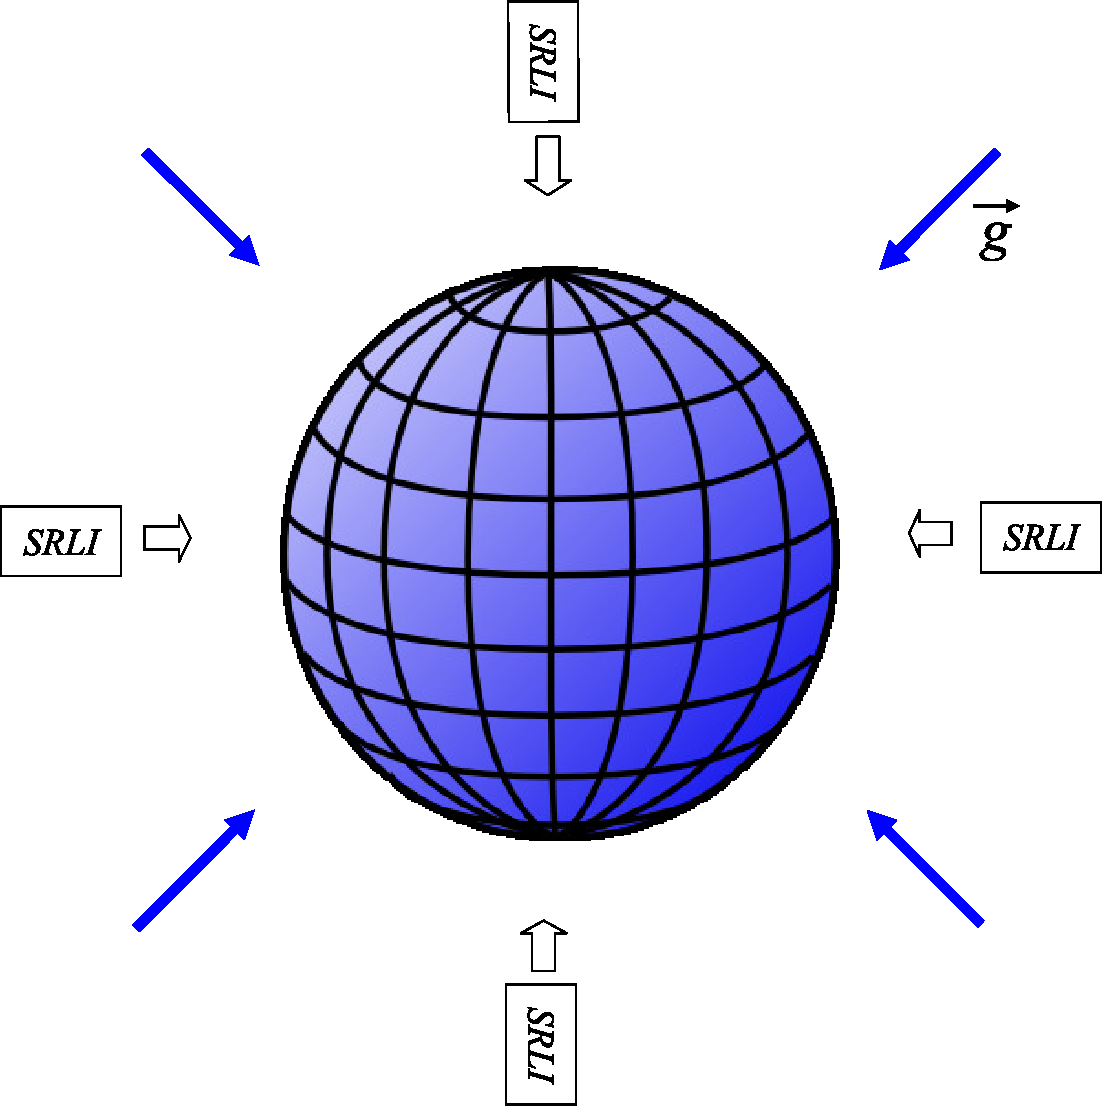
\epsfig{file=fig/fig-SRLI.pdf, width=6cm}
\caption{Sistemas de referencia localmente inerciales cayendo hacia la Tierra.}
\label{fig:SRLI}
\end{figure}

Una consecuencia directa del PEF es que \textit{la luz debiese ser deflectada por campos gravitacionales}. En efecto, la hip'otesis planteada por el PEF es que en los SRLI's, es decir, SR en caida libre, son v'alidas las leyes F'isicas conocidas en la teor'ia de RE. En particular las ecuaciones de Maxwell en su forma usual, y sus conocidas implicancias respecto de la propagaci'on de la radiaci'on electromagn'etica, son v'alidas en estos SRLI's. Como consecuencia, es en estos SRLI's en los que la luz debe(r'ia) moverse en l'inea recta con velocidad constante. 
 Por otro lado, respecto a un SR que acelera respecto a estos SRLI's, por ejemplo, en un SR a una distancia fija de la Tierra, la luz debe(r'ia) curvarse. Ver figura \ref{fig:PEF-luz}.
\begin{figure}[H]
\centering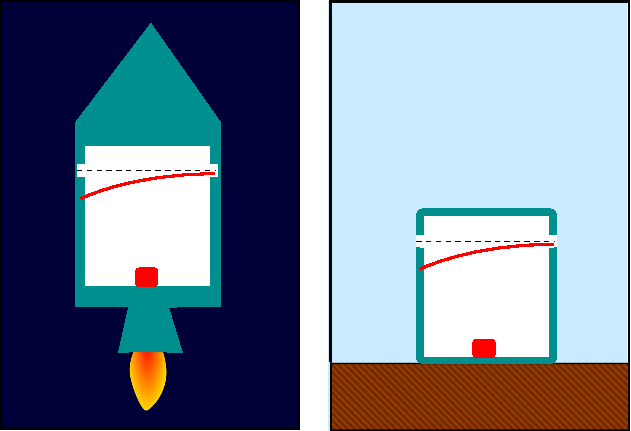
\epsfig{file=fig/fig-gravedad-y-aceleracion-luz.pdf, width=6cm}
\caption{Deflexi'on de la luz. Ambos SR's aceleran respecto a SRLI's.}
\label{fig:PEF-luz}
\end{figure}
Tal como en este caso simple, relacionado con la trayectoria de la luz en un campo gravitacional, el PEF permite determinar c'omo se comporta cualquier sistema f'isico en presencia de un campo gravitacional no nulo (en una regi'on suficientemente peque\~na), ya que es (o debe ser, de acuerdo a este principio) exactamente lo mismo que ocurre cuando el sistema se describe desde un SR que acelera respecto a uno (localmente) inercial. De hecho, el PEF \textit{unifica} localmente (los efectos de) la gravitaci'on con (los de) la aceleraci'on respectoa SRLI's, puesto que son f'isicamente indistinguibles. En este sentido en la teor'ia de gravitaci'on de Einstein la gravedad ``es'' aceleraci'on respecto a SLRI's: el hecho que en una regi'on del espacio se experimente un campo gravitacional respecto a un SR es simplemente una consecuencia de que ese SR acelera respecto a los SRLI's que cubren esa regi'on. Note que estas consideraciones son puramente ``cinem'aticas'' en el sentido que no permiten por si solas determinar la distribuci'on, orientaci'on y din'amica de los SRLI's (exactamente c'omo y hacia donde ``caen'' cada uno de estos SRLI's), 'este es precisamente el rol de las \textbf{ecuaciones de campo de la teor'ia}, que discutiremos en el cap'itulo \ref{capTEG}. No obstante, el PEF determina la forma en que un sistema f'isico responde a un campo gravitacional dado, tal como discutiremos a continuaci'on, ahora en el contexto relativista, .

\section{Observadores acelerados y gravedad: Versi'on  relativista}

Tal como Einstein \cite{Einstein56}, seguiremos considerando que un sistema coordenado (SC) est'a asociado a un SR de modo que un \textit{cambio} de SR queda descrito por una cierta \textit{transformaci'on de  coordenadas} (m'as adelante, sin embargo, veremos que es posible separar estos conceptos: un sistema de coordenadas no necesita siempre estar asociado a un sistema de referencia).

En RE la ecuaci'on que describe el movimiento de una part{\'\i}cula
en ausencia de fuerzas externas, respecto a un SRI $K$, es
\begin{equation}
\frac{d^2x^\mu}{d\tau ^2}=0, \label{tsri}
\end{equation}
donde $x^\mu(\tau )$ es la trayectoria de la part{\'\i}cula,
expresada en coordenadas (pseudo-)cartesianas $x^\mu=(ct,\vec{x})$, y donde $\tau $ es el correspondiente tiempo propio.

De acuerdo a lo discutido en las secciones anteriores, el PEF implica que (\ref{tsri}) ser'a tambi'en la ecuaci'on de movimiento de un cuerpo bajo la acci'on de la gravedad (pero libre de otras fuerzas) \textit{respecto a SRLI's}.

Deseamos ahora transformar la ecuaci'on (\ref{tsri}) para expresarla en t'erminos de las coordenadas asociadas a un SR que no sea un SRLI, es decir, un SR que \textit{acelera} respecto a los SRLI's. La transformaci'on de coordenadas correspondiente debe necesariamente ser \textit{no-lineal} (y mezclar coordenadas espaciales y temporales) para poder describir un cambio a un SR con \textit{aceleraci'on} relativa (las transformaciones de Lorentz, que describen cambios entre SR's con velocidad relativa constante, son lineales). Consideraremos entonces una \textbf{transformaci'on general de coordenadas} (TGC) $x^\mu\rightarrow \bar{x}^\mu(x)$ que en el caso considerado aqu'i describe un cambio desde el (SC asociado al) SRLI $K$ hasta (el SC asociado a) un SR $\bar{K}$ que en general no ser'a localmente inercial\footnote{El nuevo SR ser'a tambi'en localmente inercial si la transformaci'on es una transformaci'on de Lorentz. Adem'as, una TGC no s'olo puede aplicarse para describir transformaciones a SR's con movimiento relativo, sino que tambi'en al caso en que se usan \textit{coordenadas curvil'ineas en un mismo sistema de referencia}. Por ejemplo, la transformaci'on de coordenadas
$x^\mu\to\bar{x}^\mu$ con $x^\mu=(ct,x,y,z)$ y $\bar{x}^\mu=(ct,r,\theta,\varphi)$, donde $(r,\theta,\varphi)$ son las usuales coordenadas esf'ericas se interpreta
como un simple cambio de coordenadas espaciales, \textit{en el mismo SR}. En general, la TC estar'a ligada a un cambio de SR si mezcla coordenadas temporales y espaciales. Ver por ejemplo (\ref{tgan}).}. Respecto al SC $\bar{x}^\mu$ la ecuaci'on de movimiento (\ref{tsri}) adopta la forma
\begin{equation}
\boxed{\frac{d^2\bar{x}^\mu}{d\tau ^2}+\bar{\Gamma }_{\ \nu
\lambda }^\mu\frac{d\bar{x}^{\nu }}{d\tau }\frac{d\bar{x}%
^\lambda }{d\tau }=0.} \label{tsrni}\marginnote{Ec. de mov. en coord. arbitrarias}
\end{equation}
En efecto,
\begin{eqnarray}
\frac{d^2\bar{x}^\mu}{d\tau ^2} &=&\frac{d}{d\tau }\left(
\frac{d\bar{x}^\mu}{d\tau } \right) \\
&=&\frac{d}{d\tau }\left( \frac{\partial \bar{x}^\mu}{\partial x^{\nu
}}\frac{dx^{\nu }}{d\tau }\right) \\
&=&\frac{\partial \bar{x}^\mu}{\partial x^\nu } \frac{d^2x^{\nu }}{d\tau
^2}+\frac{\partial ^2\bar{x}^\mu }{\partial x^{\nu }\partial x^\lambda
}\frac{dx^\lambda }{d\tau }\frac{dx^{\nu }}{d\tau } \\
&=&\frac{\partial ^2\bar{x}^\mu }{\partial x^{\nu }\partial x^\lambda
}\frac{dx^\lambda }{d\tau }\frac{dx^{\nu }}{d\tau } \\
&=&-\bar{\Gamma }_{\ \nu
\lambda }^\mu\frac{d\bar{x}^{\nu }}{d\tau }\frac{d\bar{x}%
^\lambda }{d\tau } ,
\end{eqnarray}
donde definimos
\begin{equation}
\boxed{\bar{\Gamma }_{\ \nu\lambda }^\mu(\bar{x}):=-\frac{\partial
^2\bar{x}^\mu }{\partial x^\alpha \partial x^\beta }\frac{\partial
x^\alpha }{\partial \bar{x}^{\nu }}\frac{\partial x^\beta }{\partial
\bar{x}^\lambda }=\frac{\partial\bar{x}^\mu}{\partial x^\sigma
}\frac{\partial ^2x^\sigma }{\partial \bar{x}^{\nu }\partial \bar{x}^\lambda }.}
\label{defGammaSR}
\end{equation}
As{\'\i}, la ecuaci'on del movimiento de una part{\'\i}cula libre en un SC
general posee, adicionalmente al usual t'ermino proporcional a la
segunda derivada de la 4-posici'on, un t'ermino \textit{bilineal} en la 4-velocidad. Este segundo t'ermino describe las llamadas ``fuerzas inerciales''\footnote{'Este es el t'ermino que, en los l'imites apropiados, reproduce la aceleraci'on de Coriolis en un SR rotante, o el segundo t'ermino del lado derecho de (\ref{acelprima}).}.

Simult'aneamente, el elemento de l'inea (el tiempo propio, para el caso de separaciones tipo tiempo), adopta la forma
\begin{equation}\marginnote{Elemento de l'inea en coord. arbitrarias}
 \boxed{ds^2=\bar{g}_{\mu\nu }(\bar{x})\,d\bar{x}^\mu d\bar{x}^{\nu },}
\end{equation}
con
\begin{equation}\marginnote{m'etrica en coord. arbitrarias}
\boxed{\bar{g}_{\mu\nu }(\bar{x}):=\eta _{\lambda \rho }\,\frac{\partial x^\lambda }{\partial \bar{x}^\mu}\frac{\partial x^\rho }{\partial \bar{x}^{\nu }}.} \label{tm}
\end{equation}
Recuerde que tanto en \eqref{defGammaSR} como en \eqref{tm} las coordenadas $x^\mu$ est'an asociadas a un SRLI.

Derivando (\ref{tm}) y usando (\ref{defGammaSR}) es posible expresar las
componentes de $\bar{\Gamma }$ directamente en t'erminos de las (derivadas de las)
componentes de $\bar{g}$:
\begin{equation}
\boxed{\bar{\Gamma }_{\ \nu\lambda }^\mu\equiv \frac{1}2\bar{g}^{\mu\rho}\left(
\bar{\partial}_\nu\bar{g}_{\lambda\rho}+\bar{\partial}_\lambda\bar{g}_{\nu\rho}
-\bar{\partial}_\rho\bar{g}_{\nu\lambda}\right) ,}
\end{equation}
donde $\bar{g}^{\mu\rho}(\bar{x})$ son las componentes de la \textbf{inversa} de
$\bar{g}_{\mu\nu}(\bar{x})$, definida de modo que (en cada evento)
\begin{equation}
\bar{g}^{\mu\rho}(\bar{x})\,\bar{g}_{\rho\nu}(\bar{x})=\delta^\mu_\nu.
\end{equation}


Vemos con esto que, en peque\~nas regiones del espaciotiempo, pero respecto a SR's generales (asociados a coordenadas $\bar{x}$), los efectos del campo gravitacional sobre la trayectoria de cuerpos quedan descritos por las cantidades $\bar{\Gamma }_{\ \nu\lambda }^\mu$ (con 40 componentes linealmente independientes!) que miden ``que tan no-(localmente-)inercial'' es el SR. \textit{Simult'aneamente}, los coeficientes $\bar{g}_{\mu\nu}(\bar{x})$ que determinan el elemento de l'inea, y por consiguiente el tiempo propio, \textit{dejan de ser constantes y diagonales}  (10 componentes linealmente independientes!).

Para estudiar c'omo cambian estas cantidades entre SC's arbitrarios (es decir, ninguno de ellos asociados, en general, a SRLI's), efectuamos una segunda TGC $\bar{x}^\mu\rightarrow
\tilde{x}^\mu(\bar{x})$. Como es de esperar, se encuentra que la ecuaci'on de movimiento de la part{\'\i}cula (libre de fuerzas no-gravitacionales), expresada en coordenadas $\tilde{x}^\mu$ es nuevamente de la forma (\ref{tsrni}), es decir,
\begin{equation}
\frac{d^2\tilde{x}^\mu}{d\tau ^2}+\tilde{\Gamma }_{\ \nu
\lambda }^\mu\frac{d\tilde{x}^{\nu }}{d\tau }\frac{d\tilde{x}%
^\lambda }{d\tau }=0, \label{tsrni2}
\end{equation}
donde
\begin{eqnarray}
\tilde{\Gamma }_{\ \nu\lambda }^\mu(\tilde{x})&:=&
\frac{\partial \tilde{x}^\mu}{\partial x^\sigma }\frac{\partial
^2x^\sigma }{%
\partial \tilde{x}^{\nu }\partial \tilde{x}^\lambda } \\
&=&\frac{\partial
\tilde{x}^\mu}{\partial \bar{x}^\sigma }\frac{\partial
\bar{x}^\rho }{\partial \tilde{x}^{\nu }}\frac{\partial
\bar{x}^{\eta }}{\partial \tilde{x}^\lambda }\bar{\Gamma }_{\ \rho \eta
}^\sigma (\bar{x})+\frac{\partial \tilde{x}^\mu}{%
\partial \bar{x}^\rho }\frac{\partial ^2\bar{x}^\rho }{%
\partial \tilde{x}^{\nu }\partial \tilde{x}^\lambda }. \label{tigam} \marginnote{ley de transf. de conexi'on}
\end{eqnarray}

Vemos que los coeficientes $\Gamma$ transforman \textit{inhomog'eneamente} bajo
una TGC. Esta propiedad es precisamente la que posibilita que $\Gamma$ sea nulo
en coordenadas pseudo-cartesianas asociadas a SRLI's, pero distinto de cero en coordenadas asociadas a SR's que aceleran respecto a los primeros. M'as precisamente, los coeficientes $\Gamma$ \emph{transforman como una conexi'on} bajo una TGC.

Por otro lado, las componentes de la m'etrica en el SR $\tilde{K}$, con coordenadas $\tilde{x}$, est'an relacionadas con las componentes en $\bar{K}$ por medio de
\begin{equation}
 \tilde{g}_{\mu\nu}(\tilde{x})=\frac{\partial\bar{x}^\lambda}{\partial \tilde{x}^\mu}
\frac{\partial\bar{x}^\rho}{\partial \tilde{x}^\nu}\,\bar{g}_{\lambda\rho}(\bar{x}).  \marginnote{ley de transf. de m'etrica}
\end{equation}

M'etricas no constantes, conexiones no nulas (as'i como curvaturas y torsiones, etc.) son objetos matem'aticos definidos usualmente en el contexto de la \textit{geometr'ia diferencial} y en particular de la \textit{geometr'ia riemanniana}, o geometr'ia de \textit{espacios curvos}. En el cap'itulo \ref{cap:tensores} resumiremos algunos aspectos b'asicos de este vasto tema.

%\section{Relatividad especial y gravitaci'on newtoniana: un conflicto}
%
%En la teor'ia de la Relatividad Especial, los eventos ocurren en el
%espaciotiempo 4-dimen\-sio\-nal. Existen adem'as observadores
%``privilegiados'', los observadores inerciales. Ellos son entendidos como marcos
%infinitamente extendidos en espacio y tiempo en los que cuerpos \textit{libres}
%(que no son influenciados por ning'un otro cuerpo) se mueven con velocidad
%constante en l'ineas rectas en
%el sentido geom'etrico euclidiano. A estos SRI's asociamos un conjunto de
%coordenadas \textit{inerciales}, tambi'en llamadas (pseudo-)cartesianas,
%$x^\mu=(x^0,x^1,x^2,x^3)$. En el espacio vac'io y respecto a un SRI no existe
%preferencia entre los distintos puntos e instantes y adem'as no existe una
%direcci'on preferente. Decimos que el vac'io es invariante bajo translaciones
%(espaciales y temporales) y bajo rotaciones. Adem'as, el principio de
%relatividad establece que todos los SRI's, con velocidades relativas constantes
%entre ellos, son f'isicamente equivalentes, es decir, indistinguibles.
%Equivalentemente, las leyes f'isicas son las mismas en todos los SRI's. Esto, a
%fin de cuentas, es tambi'en una \textit{observaci'on}, es decir, una generalizaci'on de resultados experimentales. En RE estas equivalencias entre SRI's se expresan por medio de la covariancia de las ecuaciones respecto a transformaciones de Lorentz y translaciones (es decir, bajo transformaciones de Poincar\`e).
%
%Una teor'ia de la interacci'on gravitacional que sea compatible con los
%principios de la TRE (por ejemplo, con una velocidad m'axima de propagaci'on de
%las interacciones) requiere entonces que sus ecuaciones sean covariantes bajo
%TL's, es decir, que puedan ser escritas en t'erminos de vectores y tensores
%respecto a TL's.
%
%\subsection{Teor'ia escalar de la gravitaci'on*}
%La ecuaci'on newtoniana que determina el campo gravitacional es la ecuaci'on de
%Poisson (\ref{Poisson}). Una posible generalizaci'on covariante bajo TL's
%(an'aloga a la ecuaci'on que satisface el potencial electromagn'etico) es la
%ecuaci'on de onda
%\begin{equation}
%\square\phi=-4\pi G\rho, \label{casicasi}
%\end{equation}
%con $\square=\eta^{\mu\nu}\partial_\mu\partial_\nu$. En este caso la ecuaci'on
%de Poisson para el potencial $\phi$ se encuentra en el caso l'imite de campos
%est'aticos.
%
%Un primer candidato a una teor'ia relativista de la gravitaci'on podr'ia
%considerar que el campo gravitacional $\phi$ es determinado por la ecuaci'on
%(\ref{casicasi}) en el caso general en que tanto $\phi$ como $\rho$ sean
%dependientes del tiempo. Pero, ?`cu'al es el significado de la fuente $\rho$ en
%este caso?. En el caso de un fluido sin presi'on (polvo), o un conjunto de
%part'iculas puntuales donde todas las componentes se mueven con la misma
%velocidad, es posible construir un escalar proporcional a la densidad de masa
%(la densidad de masas en reposo $\rho$ vista anteriormente). Por otro
%lado, en RE la masa no es entendida como una cantidad independiente, sino
%s'olo como una componente de la energ'ia de los cuerpos. As'i,
%en una teor'ia relativista de la gravitaci'on esperamos que todo el contenido de
%energ'ia de un cuerpo aporte su a masa gravitacional. Esto significa que podemos
%intentar reemplazar densidad de masa por densidad de energ'ia como fuente del
%campo gravitacional. De este modo, para completar nuestra generalizaci'on
%(\ref{casicasi}) necesitamos una cantidad escalar bajo TL's que contenga la
%densidad de energ'ia y que se reduzca a la usual densidad de masa en los casos
%l'imites apropiados.
%
%A partir del tensor de energ'ia-mom'entum $T^{\mu\nu}$ de una distribuci'on de
%materia podemos construir el siguiente escalar:
%\begin{equation}
%T:=T^\mu_{\ \mu}=\eta_{\mu\nu}T^{\mu\nu}.
%\end{equation}
%En el caso de un fluido ideal,
%\begin{equation}
%T=\left( \rho +\frac{p}{c^2}\right) u^\mu u_\mu-p\delta^\mu_\mu=\left( \rho
%+\frac{p}{c^2}\right) c^2-4p=\rho c^2-3p.
%\end{equation}
%Para ``materia no-relativista'', $p\ll \frac{1}{3}\rho c^2$ (verificar esta
%condici'on para un gas ideal) tenemos $T=\rho c^2$, de modo que podemos
%postular
%\begin{equation}
%\square\phi=-\kappa T, \label{casicasi2}
%\end{equation}
%con $\kappa:=\frac{4\pi G}{c^2}$.
%A primera vista, lo anterior define una teor'ia relativista viable de la
%gravitaci'on. De hecho, la teor'ia es \textit{matem'aticamente consistente}. Sin
%embargo, se encontr'o que esta \textit{teor'ia escalar de la gravitaci'on no
%describe adecuadamente las observaciones}. En general, una teor'ia gravitacional
%escalar no permite describir el fen'omeno de deflecci'on de la luz por campos
%gravitacionales, debido a que un campo escalar no puede acoplarse razonablemente
%al campo electromagn'etico (ya que el tensor de enrg'ia-mom'entum
%electromagn'etico tiene traza nula). Por otro lado, hoy en d'ia la desviaci'on
%de la luz por campos gravitacionales es un hecho experimental confirmado m'as
%all'a de toda duda. En resumen, debemos considerar otras posibilidades para una
%teor'ia relativista de la gravitaci'on.
%

